
% Default to the notebook output style

    


% Inherit from the specified cell style.




    
\documentclass[float=false,crop=false]{standalone}

    
    
\usepackage{../myipy2tex}  % NOTE WE ARE ASSSUMING THE STYLE FILE TO BE ONE FOLDER ABOVE

% if you need to cross reference to any raw tex file from this resultant tex file you  need to refer them here..
% it is not needed when you compile main.tex but make sure the labels are unique
\IfEq{\jobname}{\detokenize{main}}{}{%
    \externaldocument{raw_sample} 
} 




    


    


    \begin{document}
    
    
    \maketitle
    
    

    
    \section{Sample}\label{sample}

This is just a sample notebook

\subsection{Sample Sub Section}\label{sample-sub-section}

   \begin{Verbatim}[commandchars=\\\{\},fontsize=\scriptsize]
{\color{incolor}In [{\color{incolor}1}]:} \PY{n+nb}{print}\PY{p}{(}\PY{l+m+mi}{3}\PY{o}{+}\PY{l+m+mi}{4}\PY{p}{)}
\end{Verbatim}

    \begin{Verbatim}[commandchars=\\\{\},fontsize=\footnotesize]
7

    \end{Verbatim}

    \textbf{Issues:}

The \texttt{subsubsections} are not numbered. At this time, it looks
like problem is at least outside the scope of ipython as even raw tex
file shows this problem. Try limiting your sections to 2 levels only.
That is till \texttt{\#\#} not beyond to be on safe side.

\subsection{this subsection is
numbered}\label{this-subsection-is-numbered}

\subsubsection{this subsubsection is not
numbered}\label{this-subsubsection-is-not-numbered}

    \subsection{Using Latex Equations}\label{using-latex-equations}

Latex equations cause few issues because Mathjax used by ipython is not
fully latex compliant.

\textbf{Issues:}

\begin{enumerate}
\def\labelenumi{\arabic{enumi}.}
\tightlist
\item
  Mathjax is lineant on not using brackets to cover multi digit
  subscripts while latex is not.
  \texttt{\textbackslash{}mu\_\textbackslash{}widehat\{p\}} will be
  converted properly in notebook while gives error in converted tex
  file. Always wrap subscripts fully. For eg,
  \texttt{\textbackslash{}mu\_\{\textbackslash{}widehat\{p\}\}} will
  work in tex as well.
\item
  If you use \texttt{begin\{equation\}}, need not embrace further with
  \texttt{\$\$} which will only create error in converted tex.
\item
  \texttt{begin\{equation\}} does not allow multi line, so use
  \texttt{begin\{aligned\}} inside.
\item
  Double slash for new line will not work unless the set of equations
  are wrapped within \texttt{\textbackslash{}begin\{align\}}
\end{enumerate}

References: \href{https://github.com/jupyter/nbconvert/issues/881}{1}

\textbf{Demo:}

Set of latex equations which successfully works in converted tex as
well.

Raw:

\begin{verbatim}
$$
\color{blue}{
\begin{aligned}
    \text{Random Variable} \ \ \widehat{p} =  \overline{\widehat{Y}} \\
    \mu_{\widehat{p}} = \mu{\overline{\widehat{Y}}} \\
    \sigma_{\widehat{p}} = \sigma(\overline{\widehat{Y}})
\end{aligned}
}
$$
\end{verbatim}

Output: \[
\color{blue}{
\begin{aligned}
    \text{Random Variable} \ \ \widehat{p} =  \overline{\widehat{Y}} \\
    \mu_{\widehat{p}} = \mu{\overline{\widehat{Y}}} \\
    \sigma_{\widehat{p}} = \sigma(\overline{\widehat{Y}})
\end{aligned}
}
\]

Raw:

\begin{verbatim}
$$
\begin{equation}
\color{blue}{
\begin{aligned}
    \text{Random Variable} \ \ \widehat{p} =  \overline{\widehat{Y}} \nonumber \\ \\
    \mu_{\widehat{p}} = \mu{\overline{\widehat{Y}}} \nonumber \\ \\
    \sigma_{\widehat{p}} = \sigma(\overline{\widehat{Y}}) \nonumber 
\end{aligned}}
\end{equation}
$$
\end{verbatim}

Output (note even if I give nonumber, equation is numbered!):

\begin{equation}
\color{blue}{
\begin{aligned}
    \text{Random Variable} \ \ \widehat{p} =  \overline{\widehat{Y}}  \\ \\
    \mu_{\widehat{p}} = \mu{\overline{\widehat{Y}}}  \\ \\
    \sigma_{\widehat{p}} = \sigma(\overline{\widehat{Y}}) 
\end{aligned}}
\end{equation}

    \subsection{Using Attachments}\label{using-attachments}

\textbf{Issue:}\\
Using a \texttt{backslash\ and\ a\ space\ and\ then\ a\ blank\ line} to
avoid attachments becoming floats and placed out of section. This is to
be done after every attachment. Else they simply float around. This is a
latex issue. Do not worry, they will not appear in latex though they
appear here. If nbconvert did not use figure and instead only
includegraphis this issue could have been avoided. Got this hint from
\href{https://tex.stackexchange.com/questions/101725/latex-figures-appear-before-text-in-pandoc-markdown/101726}{here}

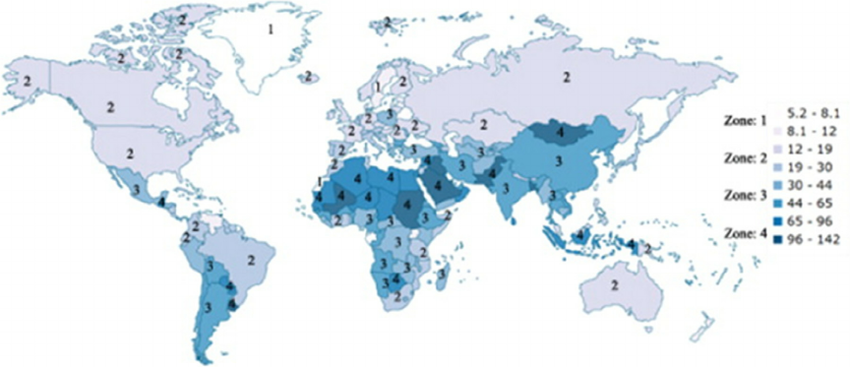
\includegraphics{ipy_sample_files/attach_4_image.png} ~

    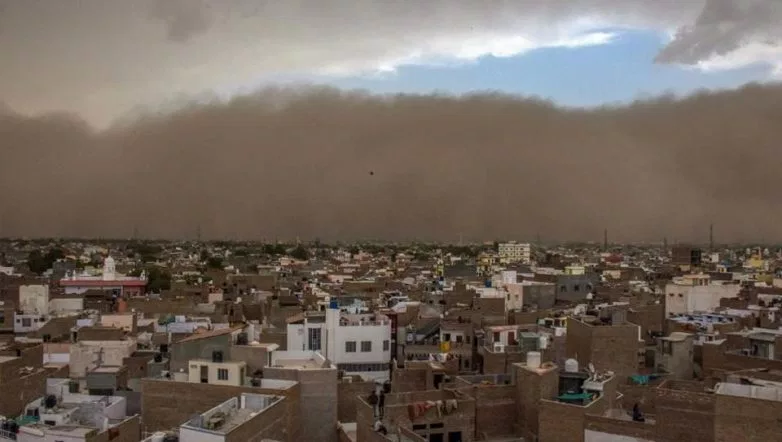
\includegraphics{ipy_sample_files/attach_5_image.png} ~

    \subsection{Using Code}\label{using-code}

This so far seem to have no problems

   \begin{Verbatim}[commandchars=\\\{\},fontsize=\scriptsize]
{\color{incolor}In [{\color{incolor}3}]:} \PY{o}{\PYZpc{}}\PY{k}{matplotlib} inline
        \PY{k+kn}{import} \PY{n+nn}{matplotlib}\PY{n+nn}{.}\PY{n+nn}{pyplot} \PY{k}{as} \PY{n+nn}{plt}
        
        \PY{n}{x} \PY{o}{=} \PY{p}{[}\PY{l+m+mi}{1}\PY{p}{,}\PY{l+m+mi}{2}\PY{p}{,}\PY{l+m+mi}{3}\PY{p}{,}\PY{l+m+mi}{4}\PY{p}{,}\PY{l+m+mi}{5}\PY{p}{]}
        \PY{n}{y} \PY{o}{=} \PY{p}{[}\PY{l+m+mi}{2}\PY{p}{,}\PY{l+m+mi}{4}\PY{p}{,}\PY{l+m+mi}{6}\PY{p}{,}\PY{l+m+mi}{8}\PY{p}{,}\PY{l+m+mi}{10}\PY{p}{]}
        \PY{n}{plt}\PY{o}{.}\PY{n}{plot}\PY{p}{(}\PY{n}{x}\PY{p}{,}\PY{n}{y}\PY{p}{)}
        \PY{n}{plt}\PY{o}{.}\PY{n}{show}\PY{p}{(}\PY{p}{)}
\end{Verbatim}

    \begin{center}
    \adjustimage{max size={0.9\linewidth}{0.9\paperheight}}{ipy_sample_files/ipy_sample_7_0.png}
    \end{center}
    { \hspace*{\fill} \\}
    
    \subsection{Cross Reference}\label{cross-reference}

Sometimes you would want to refer an equation or something in another
tex file from here. This is how to do it.

This \ref{ch:chapter_1} is a sample cross reference to a section in another raw tex file. 
This \ref{eq:1} is a sample cross reference to an equation in another raw tex file.

    \textbf{Issue:} We need to do this in raw cell as cross references are
not realized at nbconvert level. Also using this externaldocument would
compile the entire main.tex file currently instead of only the
referenced file. This should be investigated why. Its a nuisance for
now. Also note the line breaks explicitly given instead of double space
or latex break because these are raw cells, so a line break also should
be literally given as above (would be clear when you view this document
in notebook)


    % Add a bibliography block to the postdoc
    
    
    
    \end{document}
